\chapter{Mise en place de l’interface utilisateur}
\subsection{Transmettre le savoir métier}
L’arrivée du développeur dans les réflexions autour de cette nouvelle fonctionnalité met en lumière le travail indispensable de transmission du savoir métier aux personnes non-archivistes de l’équipe. En effet, il est essentiel pour le profil métier de l’équipe, ici la \textit{\gls{Product Owner}} et archiviste ainsi que la stagiaire chargée d'expertise fonctionnelle, de s’assurer que tout le monde a conscience de la culture métier des utilisateurs de cette fonctionnalité. Néanmoins, en ce qui concerne le périmètre de notre fonctionnalité, transmettre l’ensemble des savoirs nécessaires à la pleine compréhension du besoin n’est pas évident. Il a fallu présenter à l’aide d’un exemple la chaîne de traitement détaillée en partie 1 de ce mémoire ainsi que le fonctionnement global de ses outils. Il est également indispensable de transmettre quelques notions d’archivistique et notamment d’expliquer qu’\gls{Archifiltre} ne travaille pas sur les originaux mais sur une image des fichiers afin de garantir l’intégrité des archives. En effet, pour des non-archivistes, ce fait qui empêche par exemple le renommage possible dans \gls{Archifiltre} de s’appliquer sur les originaux, est un point de frustration et d’incompréhension qu’il est nécessaire d’expliquer. Il est également indispensable de transmettre le vocabulaire archivistique mais aussi les notions de \gls{SIP} et de \gls{SAE} relativement complexes à appréhender. Cette étape est d’autant plus importante que le développeur d’\gls{Archifiltre} est qualifié en \textit{UX design} et prend donc part à la définition de l’interface utilisateur. 


Par ailleurs, la plus grande difficulté de transmission, y compris avec quelqu’un de techniquement très qualifié, reste principalement le \gls{SEDA}. Ceci peut notamment s’expliquer par le fait qu’il réponde à des problématiques très précises d’archivistique, parfois même trop spécifiques pour la plupart des archivistes. Nous pouvons également noter que la documentation du \gls{SEDA} reste relativement difficile d’accès et pauvre\footnote{Une nouvelle documentation est néanmoins en cours de préparation et devrait être accessible en décembre 2024.}. Une partie est disponible sur FranceArchives mais se trouve majoritairement sur Github\footcite{noauthor_culturecommunicationseda_2024}, ce qui rend son accès complexe pour un certain nombre d’archivistes. Par ailleurs, le dictionnaire du \gls{SEDA} 2.2\footcite{siaf_dictionnaire_2022}, document selon moi le plus utile pour appréhender le \gls{SEDA} et la logique de son schéma, est construit de telle manière qu’il est difficile de comprendre la hiérarchie concrète des balises et la forme que prend finalement un \textit{\gls{manifest}}. Afin de pallier ces difficultés, nous avons construit un double tableau en nous limitant aux balises pouvant être enrichies pour chaque unité d’archive avec les informations extraites d’un système d’information c’est-à-dire l’ensemble des balises de la balise <content>, métadonnées de description, et de la balise <management>, métadonnées de gestion, pour chaque unité d’archive (<archiveunit>). Le double tableau produit retranscrit les niveaux de hiérarchie des balises et leur associe une traduction française, leur niveau de répétabilité et d’obligation, leur type, leur définition ainsi que des informations particulières à certaines balises comme la liste de termes lorsqu’il s’agit de balises qui n’acceptent qu’une liste de termes définis. Ce document est particulièrement important car il servira ensuite d’appui au développeur pour construire la partie \textit{\gls{mapping}} \gls{SEDA} de la fonctionnalité. Il est consultable en annexes \ref{annexeb} et \ref{annexec}. 


\subsection{Définition des \textit{wireframes} et évolution d’après les retours utilisateurs}

A partir de toutes ces informations et des retours des différents échanges avec les utilisateurs effectués jusque là, le travail de la définition des \textit{\gls{wireframe}s} commence. La première étape consiste à effectuer un \textit{\gls{benchmark}} des interfaces notamment proposées sur le site \textit{Mobbin}\footnote{\href{https://mobbin.com/}{https://mobbin.com/}} et des produits étudiés dans le premier \textit{\gls{benchmark}} mais en l’élargissant à une réflexion uniquement orientée sur l’interface utilisateur (\gls{UI}). Ce \textit{\gls{benchmark}} nous mène à la création des premiers \textit{\gls{wireframe}s} des différents écrans du processus. 


Un \textit{\gls{wireframe}}, ou maquette fonctionnelle, est un schéma qui permet de définir les zones et les différents composants de chaque fenêtre de l’interface utilisateur de notre fonctionnalité. Pour les construire, nous utilisons l’outil \textit{Balsamiq}\footnote{ \href{https://balsamiq.com/}{https://balsamiq.com/}} qui imite le papier et le crayon, fonction importante pour la définition de \textit{\gls{wireframe}s} car le design graphique doit rester absent de cette étape afin de concentrer les réflexions sur l’essentiel. Cet outil permet également de simuler des interactions et de naviguer entre les \textit{\gls{wireframe}}, recréant ainsi le parcours conçu à l'étape précédente. Cette fonctionnalité facilite les tests utilisateurs car elle met en place des conditions un minimum réelles aidant ainsi les utilisateurs à se projeter. En effet, un des points d’attention lorsque l’interface utilisateur est testée est de noter où l’utilisateur clique instinctivement et ce qu’il comprend de l’interface. 


Dans notre cas, il était nécessaire de définir des \textit{\gls{wireframe}s} pour huit étapes du processus : 
\begin{itemize}
	\item La fenêtre d’\gls{Archifiltre} actuelle avec un bouton d’import de métadonnées, 
	\item Une fenêtre de messages de rappel des contraintes à respecter pour l’import,
	\item Une fenêtre d’import du CSV de métadonnées, 
	\item Une fenêtre de sélection de la clé de jointure,  
	\item Une fenêtre qui permet de choisir d’importer ou non chaque métadonnée, 
	\item Une fenêtre de vérification afin de s’assurer de la bonne jointure des données, 
	\item Un nouvel onglet de visualisation tableur des métadonnées importées,  
	\item Une fenêtre qui permet de faire le \textit{\gls{mapping}} avec les balises \gls{SEDA}. 
\end{itemize}
Pour chacun de ces \textit{\gls{wireframe}s}, l’équipe a produit une version puis a fait passer un test utilisateur qui a permis de faire évoluer ces versions. Un autre test a ensuite permis de mettre à l’épreuve les nouvelles versions et de les faire évoluer de nouveau. Cette méthode a été effectuée pour cinq tests utilisateurs jusqu’à obtenir une version répondant à la majorité des blocages rencontrés par les différents utilisateurs. Ainsi, un grand nombre de \textit{\gls{wireframe}s} ont été produits pour aboutir à celles définissant les huit étapes susmentionnées. 


Au cours de ces évolutions, la fenêtre permettant de choisir la colonne de métadonnées du CSV importé correspondant au chemin, jointure imposée pour ce \gls{MVP}, a disparu. Elle est remplacée par l’exigence d’importer un CSV dont la première colonne contient le chemin des fichiers. Cette exigence est indiquée dans la fenêtre de message de rappel qui se présente comme une liste à cocher de quelques consignes à respecter comme le format CSV ou le format des dates importées. Soumettre l’import au fait de cocher les cases est le choix qui a été fait à l’issue de l’ensemble de tests utilisateurs afin de garantir le fait que ces indications soient prises en compte. 

\clearpage

\begin{figure}[h]
	\centering
	\begin{minipage}[b]{0.45\textwidth} %Crée une sous-structure dans le document qui prend ici 45% de la largeur totale de la ligne.
		\centering
		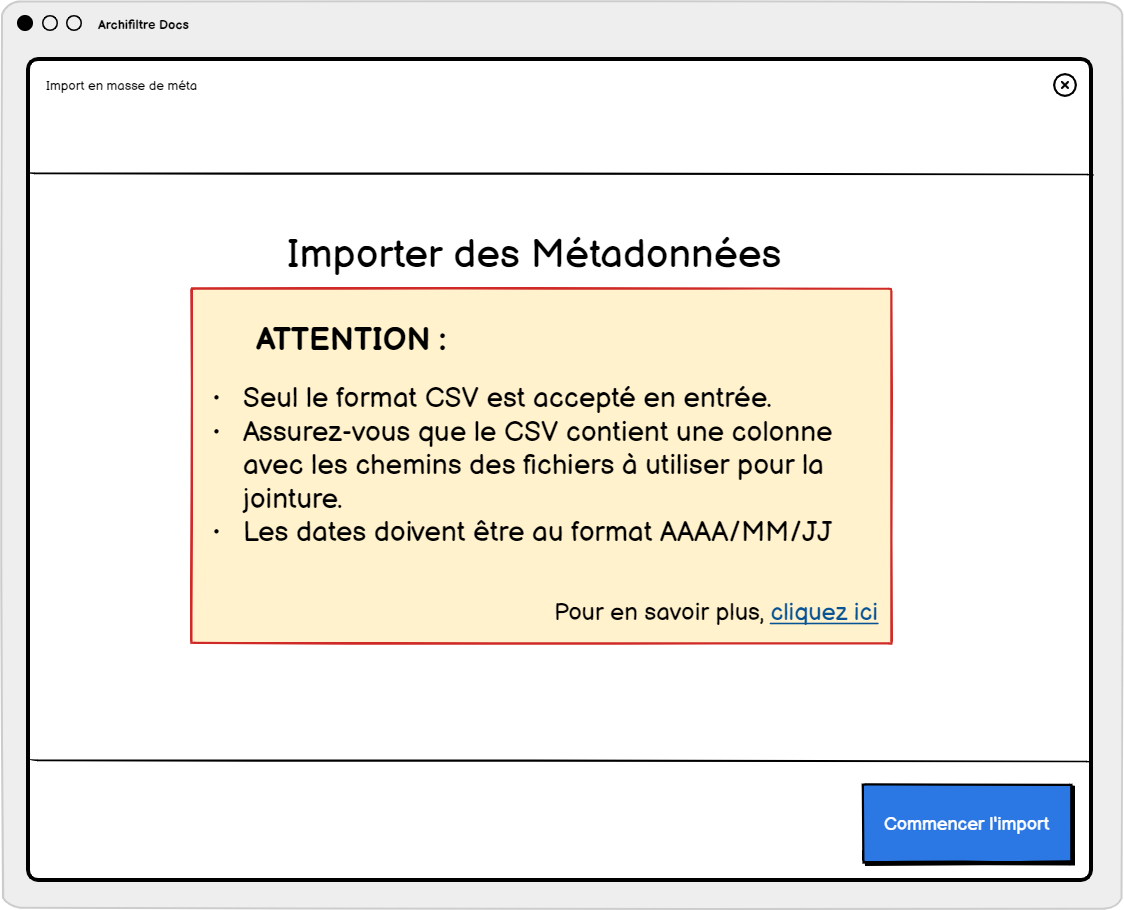
\includegraphics[width=\textwidth]{illustrations/figure21.png}
		\caption{Première version}
		\label{figure21}
	\end{minipage}
	\hfill %Met un espace entre les deux images.
	\begin{minipage}[b]{0.45\textwidth}
		\centering
		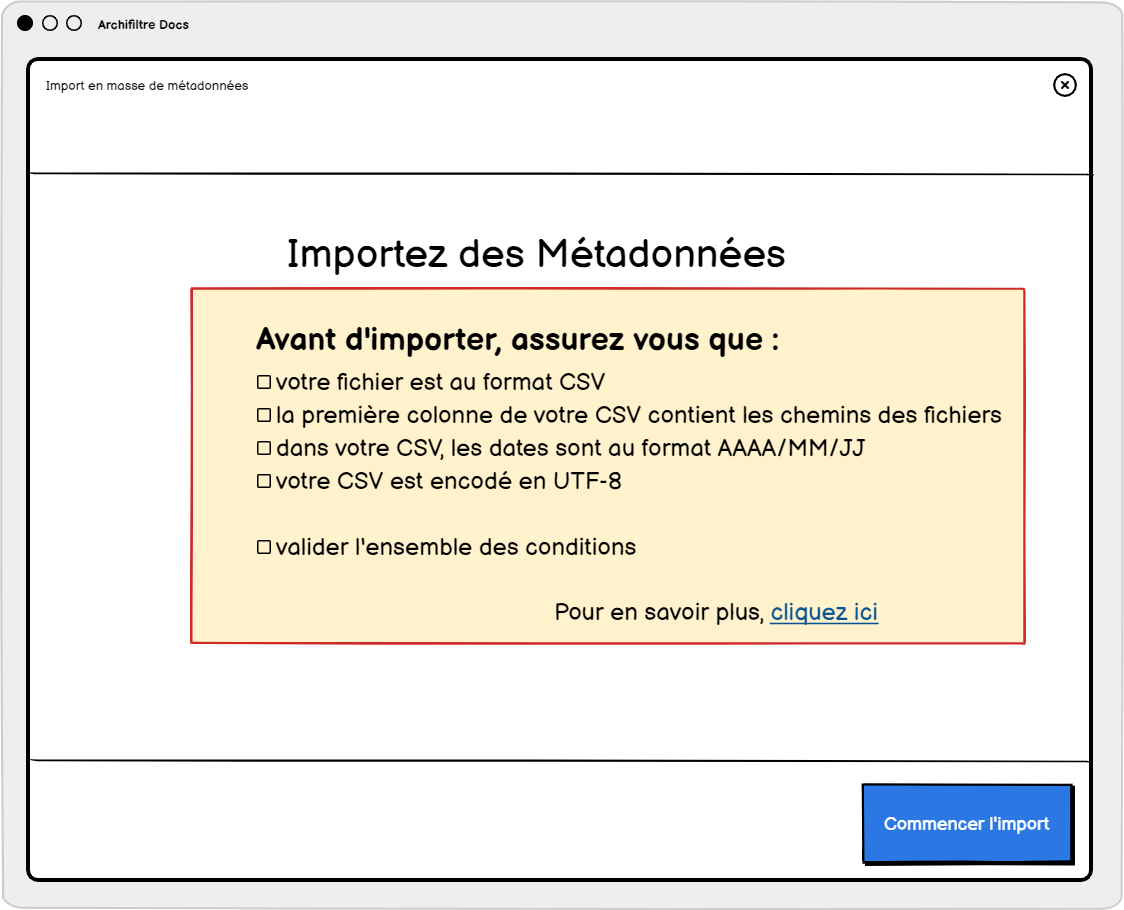
\includegraphics[width=\textwidth]{illustrations/figure22.png} 
		\caption{Version finale}
		\label{figure22}
	\end{minipage}
	\caption{Evolution des \textit{\gls{wireframe}s} de la fenêtre de vérification des contraintes à respecter avant import du CSV de métadonnées }
	\label{fig:sidebyside2}
\end{figure}


Pour présenter un cas plus détaillé d’évolution d’un \textit{\gls{wireframe}}, nous pouvons prendre l’exemple du \textit{\gls{wireframe}} le plus complexe à concevoir, celui permettant l’association de chaque métadonnée à une balise \gls{SEDA}.  La première version de ce \textit{\gls{wireframe}} s’inspirait de ce que propose ReSIP et proposait des escaliers de menus déroulants pour soit les métadonnées de gestion, soit les métadonnées de description. 

\clearpage

\insererImage{0.4}{illustrations/figure23.png}{Première version du \textit{\gls{wireframe}} d’association des métadonnées avec des balises \gls{SEDA}}{figure23}


Les tests utilisateurs et notamment celui d’Anne Lambert ont permis de faire ressortir les faiblesses de cette proposition, à savoir les difficultés de lisibilité pour les balises ayant un certain niveau de profondeur, quatre étant le nombre maximum. C’est par exemple le cas ci-dessus avec la balise <City>, sous-balise de <BirthPlace>, elle-même sous-balise de <Signer>, elle-même sous-balise de <Signature>, qui est une balise de <Content>, c'est-à-dire une métadonnée de description. Sa deuxième problématique réside dans le fait qu’une telle logique demande à l’utilisateur d’avoir préalablement une idée d’où aller chercher sa balise puisque les sous-balises n’apparaissent pas immédiatement. Anne Lambert nous a alors indiqué sa préférence pour une barre de recherche proposant de l’autocomplétion et associant le nom de la balise au chemin des balises dans laquelle elle se trouve comme le présente le \textit{\gls{wireframe}} suivant : 

\clearpage

\insererImage{0.4}{illustrations/figure24.png}{Deuxième version du \textit{\gls{wireframe}} d’association des métadonnées avec des balises \gls{SEDA}}{figure24}


A partir de cette idée, l’équipe a poursuivi les réflexions et a choisi de s’inspirer d'une interface, trouvée dans le cadre de nos recherches, qui semblait adaptée au besoin\footnote{Pour consulter l’interface : \href{https://baymard.com/ux-benchmark}{https://baymard.com/ux-benchmark}} et du double tableau présentant les sous-balises de <content> et de <management> présenté précédemment\footnote{Lien vers le double tableau en annexes \ref{annexeb} et \ref{annexec}} pour produire la version préférée des utilisateurs interrogés présentée ci-dessous. Ce \textit{\gls{wireframe}} propose pour chaque métadonnée à la fois une barre de recherche avec autocomplétion comme présenté dans le  \textit{\gls{wireframe}} précédent et à la fois une version améliorée des menus déroulants, présentant le nombre de sous-balise de chaque balise à tous les niveaux et reprenant les informations de définition de la balise, de répétabilité, de type et indiquant s’il s’agit d’une balise obligatoire comme cela a été mis en forme dans le double tableau des balises \gls{SEDA}. Par ailleurs, cette version propose deux options demandées par les utilisateurs : la possibilité de passer des noms de balises en français aux noms de balises en anglais ainsi que la possibilité de sauvegarder le balisage et ainsi de pouvoir l’effectuer de manière discontinue. 

\clearpage

\insererImage{0.35}{illustrations/figure25.png}{Version finale du \textit{\gls{wireframe}} d’association des métadonnées avec des balises \gls{SEDA}}{figure25}


\clearpage

Suivant cet exemple, un travail similaire, largement aidé des tests utilisateur, a été fait pour chaque \textit{\gls{wireframe}}. Cela a permis de fixer l’ensemble des \textit{\gls{wireframe}s} du processus de cette fonctionnalité d’import de métadonnées\footnote{Pour consulter le parcours de wireframes validés, voir annexe \ref{annexe9}}.

L’interface utilisateur du processus de la fonctionnalité d’import de métadonnées fixé, la prochaine étape consiste alors à commencer son développement. 
